\chapter{Gráficos do Experimento 3}
\subsubsection{Algoritmo Genético Geracional Clásico}

\begin{figure}[H]
\centering

\includegraphics[scale=1]{apxC/aggc/1}

\end{figure}

\begin{figure}[H]
\centering

\includegraphics[scale=1]{apxC/aggc/2}

\end{figure}

\begin{figure}[H]
\centering

\includegraphics[scale=1]{apxC/aggc/3}

\end{figure}

\begin{figure}[H]
\centering

\includegraphics[scale=1]{apxC/aggc/4}

\end{figure}

\begin{figure}[H]
\centering

\includegraphics[scale=1]{apxC/aggc/5}

\end{figure}

\begin{figure}[H]
\centering

\includegraphics[scale=1]{apxC/aggc/6}

\end{figure}

\begin{figure}[H]
\centering

\includegraphics[scale=1]{apxC/aggc/7}

\end{figure}

\begin{figure}[H]
\centering

\includegraphics[scale=1]{apxC/aggc/8}

\end{figure}

\begin{figure}[H]
\centering

\includegraphics[scale=1]{apxC/aggc/9}

\end{figure}

\begin{figure}[H]
\centering

\includegraphics[scale=1]{apxC/aggc/10}

\end{figure}

Algoritmo Genético de Regime Permanente

\begin{figure}[H]
\centering

\includegraphics[scale=1]{apxC/agrpc/1}

\end{figure}

\begin{figure}[H]
\centering

\includegraphics[scale=1]{apxC/agrpc/2}

\end{figure}
\begin{figure}[H]
\centering

\includegraphics[scale=1]{apxC/agrpc/3}

\end{figure}
\begin{figure}[H]
\centering

\includegraphics[scale=1]{apxC/agrpc/4}

\end{figure}
\begin{figure}[H]
\centering

\includegraphics[scale=1]{apxC/agrpc/5}

\end{figure}
\begin{figure}[H]
\centering

\includegraphics[scale=1]{apxC/agrpc/6}

\end{figure}
\begin{figure}[H]
\centering

\includegraphics[scale=1]{apxC/agrpc/7}

\end{figure}
\begin{figure}[H]
\centering

\includegraphics[scale=1]{apxC/agrpc/8}

\end{figure}
\begin{figure}[H]
\centering

\includegraphics[scale=1]{apxC/agrpc/9}

\end{figure}
\begin{figure}[H]
\centering

\includegraphics[scale=1]{apxC/agrpc/10}

\end{figure}